\subsection{Auswertung zu V501}


Die gemessenen Werte für die Beschleunigungsspannung $U_{B}$, die Ablenkung des Elektronenstrahls $D$ und die Ablenkspannung $U_{\text{d}}$ sind in der Tabelle
\ref{tab:V501} aufgeführt.
%\documentclass[captions=tableheading]{scrartcl}
%\usepackage{booktabs}
%\usepackage{pdflscape}




%\begin{document}
%\begin{landscape}


\begin{table}[h!]
  \centering
  \caption{Messergebnisse $U_\text{d}$ und D in Abhängigkeit von $U_B$}
  \label{tab:V501}
  \begin{tabular}{c c c c c c c c c c}
    \toprule
    \multicolumn{2}{c}{$U_B = 150V $} &   \multicolumn{2}{c}{$U_B = 250V$}&    \multicolumn{2}{c}{$U_B = 350V$}& \multicolumn{2}{c}{$U_B = 450V$}&  \multicolumn{2}{c}{$U_B = 480$}\\
      \midrule
    $U_\text{d}$ & $\text{D}$ & $U_\text{d}$ & $\text{D}$ & $U_\text{d}$ & $\text{D}$ & $U_\text{d}$ & $\text{D}$ & $U_\text{d}$ & $\text{D}$\\
      V &     cm &   V &     cm &   V &    cm  &  V  &  cm    &  V  & cm \\
    \midrule

    -7,3&			 1,5875& -12,3	&				 1,524& 16,4&					 1,4478 & -19,7&					 1,3462 & -&-\\
    -4,5&			 0,9525& -7,5 	&				 0,889& 10,5&					 0,8128 & -11,3&					 0,7112 & -10,6&					 0,635\\
    -1,6&			 0,3175& -2,7 	&				 0,254& -3,7&					 0,1778 &   -2,9&					 0,0762 &   -0,9&					 0,0\\
     1,1&			-0,3175&  2,4	  &				-0,381&  2,9&					-0,4572 &    6,4&					-0,5588 &    8,6&					-0,635\\
     3,6&			-0,9525&  6,9	  &				-1,016&  9,8&					-1,0922 &   13,6&					-1,1938 &   17,9&					-1,27\\
     6,2&			-1,5875& 11,4	  &				-1,651& 15,7&					-1,7272 &   21,6&					-1,8288 &   27,0&					-1,905\\
     8,8&			-2,2225& 16,2	  &				-2,286& 22,6&					-2,3622 &   29,6&					-2,4638 & -     &-           \\
     11,4&		-2,8575& 20,8	  &				-2,921& 28,8&					-2,9972 &      -&            -    &   -    & -     \\
     14,0&		-3,4925& 25,6	  &				-3,556& 34,4&					-3,6322 &     - &             -   &    -   &-      \\
    \bottomrule
  \end{tabular}
\end{table}

%\end{landscape}
%\end{document}

In den Abbildungen \ref{fig:150V}, \ref{fig:250V}, \ref{fig:350V}, \ref{fig:450V} und \ref{fig:480V} wird $D$ gegen $U_{\text{d}}$ aufgetragen.

\begin{figure}[h!]
  \centering
  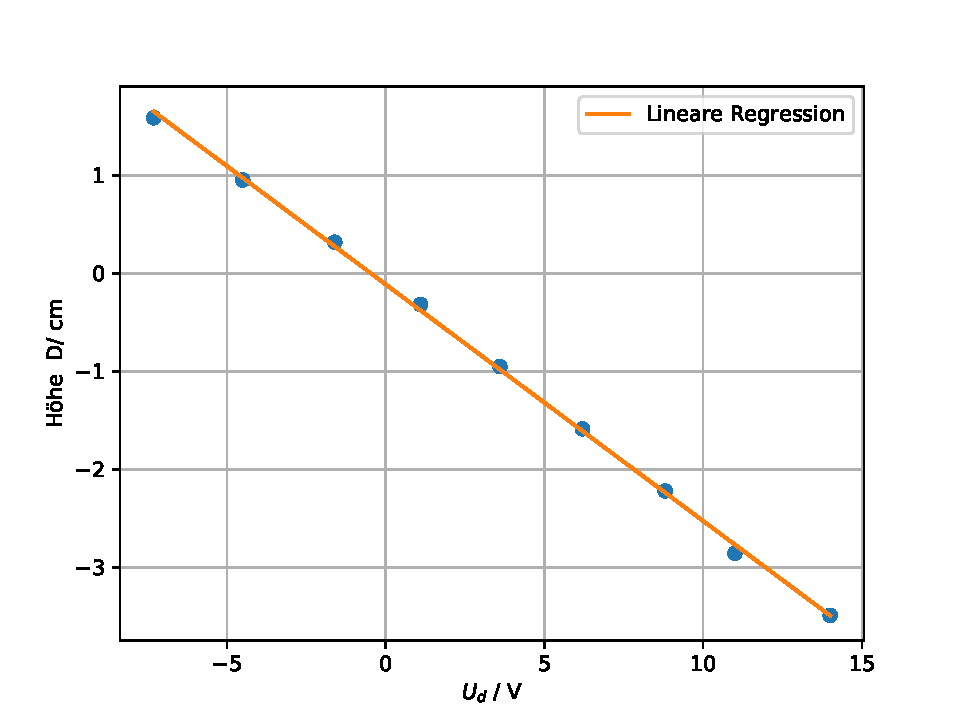
\includegraphics[width=0.8\textwidth]{150V.pdf}
  \caption{Höhe D gegen $U_{\text{d}} f\ddot{u}r 150V$}
  \label{fig:150V}
\end{figure}

\begin{figure}[h!]
 \centering
 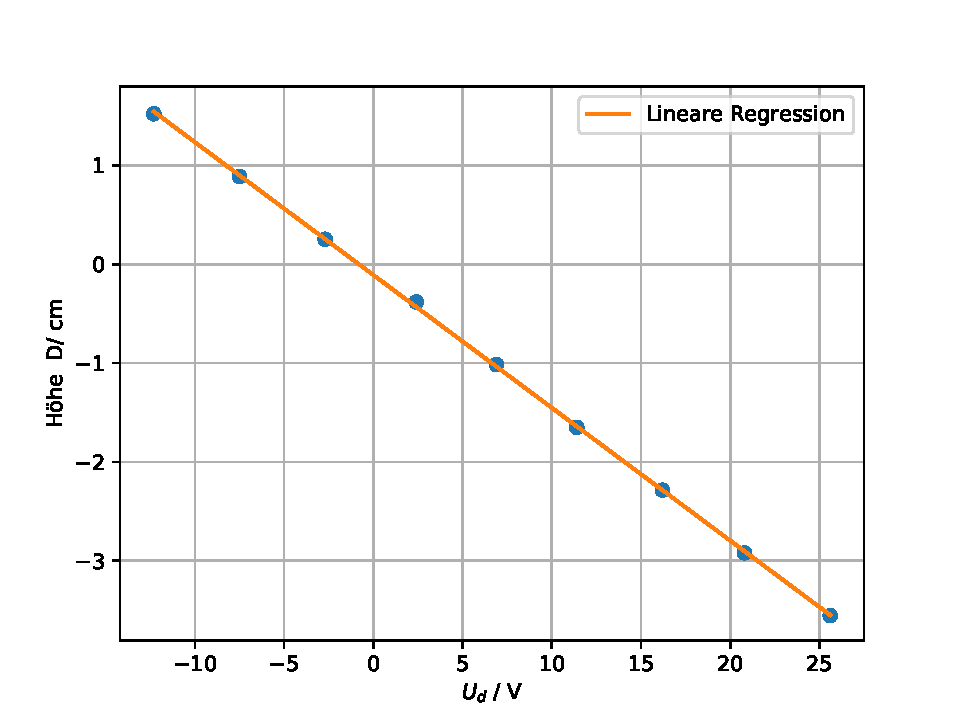
\includegraphics[width=0.8\textwidth]{250V.pdf}
 \caption{Höhe D gegen $U_{\text{d}} f\ddot{u}r 250V$}
 \label{fig:250V}
\end{figure}

\begin{figure}[h!]
  \centering
  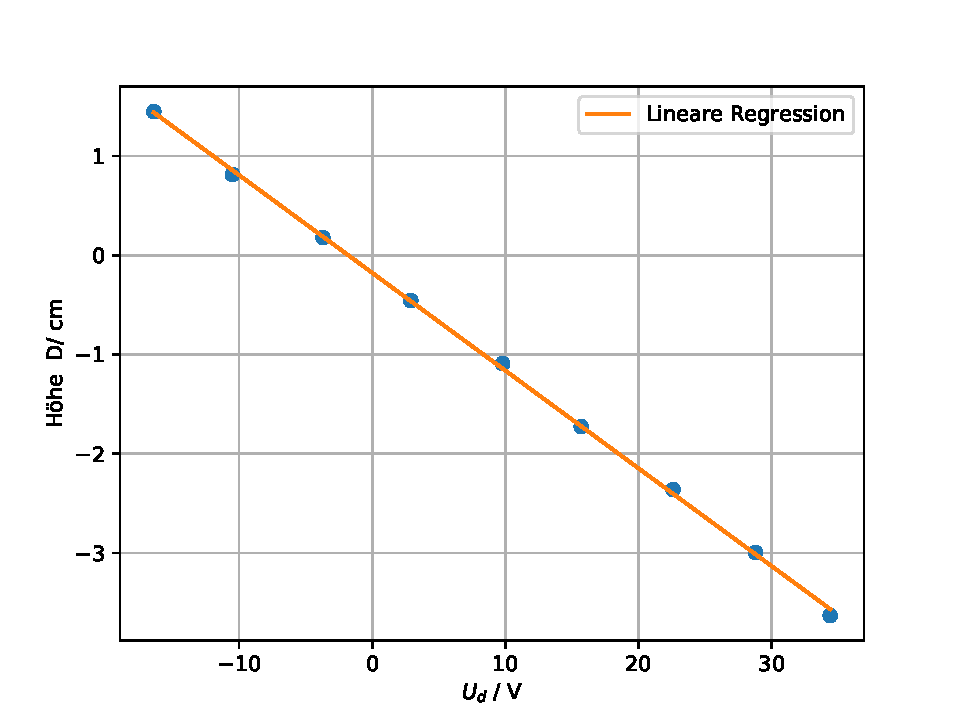
\includegraphics[width=0.8\textwidth]{350V.pdf}
  \caption{Höhe D gegen $U_{\text{d}} f\ddot{u}r 350V$}
  \label{fig:350V}
\end{figure}

\begin{figure}[h!]
  \centering
  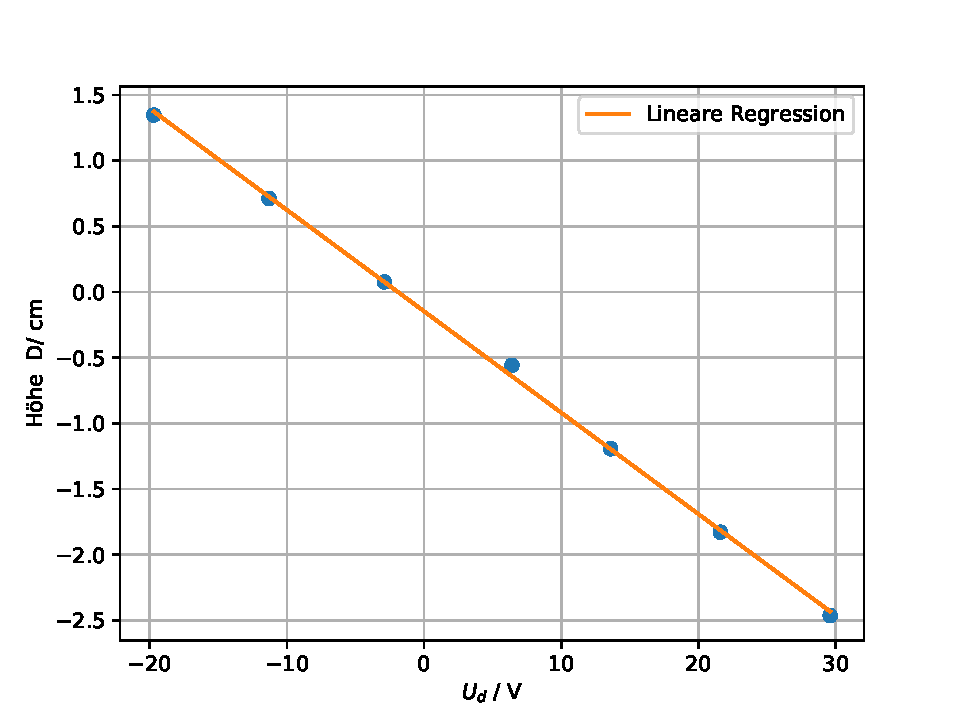
\includegraphics[width=0.8\textwidth]{450V.pdf}
  \caption{Höhe D gegen $U_{\text{d}} f\ddot{u}r 450V$}
  \label{fig:450V}
\end{figure}

\begin{figure}[h!]
  \centering
  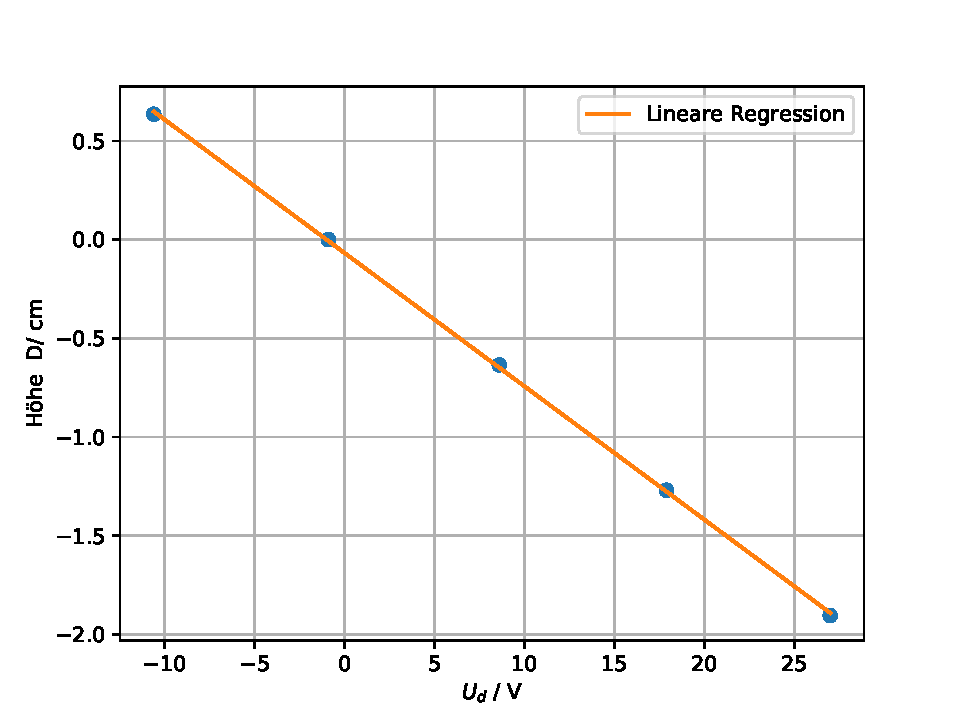
\includegraphics[width=0.8\textwidth]{480V.pdf}
  \caption{Höhe D gegen $U_{\text{d}}  f\ddot{u}r  480V$}
  \label{fig:480V}
\end{figure}
\begin{align*}
  150V\\
  Steigung:   (-0.24155702\pm6.70315714\cdot10^{-6})\si{\frac{cm}{V}}\\
  Y-Achse:    (-0.11241836\pm3.89639666\cdot10^{-4})\si{cm}
\end{align*}


\begin{align*}
  250V\\
  Steigung: (-0.13446489\pm4.13337095\cdot10^{-7})\si{\frac{cm}{V}}\\
  Y-Achse:  (-0.10761495\pm8.03068033\cdot10^{-5})\si{cm}
\end{align*}


\begin{align*}
350V\\
Stiegung: (-0.09853167\pm6.37684729\cdot10^{-7})\si{\frac{cm}{V}}\\
Y-Achse:  (-0.17695027\pm2.31507889\cdot10^{-4})\si{cm}
\end{align*}

\begin{align*}
450V\\
Steigung: (-0.07717596\pm9.45031190\cdot10^{-7})\si{\frac{cm}{V}}\\
Y-Achse:  (-0.14756239\pm2.82541359\cdot10^{-4})\si{cm}
\end{align*}

\begin{align*}
480V\\
Steigung: (-0.06754249\pm2.40937941\cdot10^{-7})\si{\frac{cm}{V}}\\
Y-Achse:  (-0.06764309\pm5.95858844\cdot10^{-5})\si{cm}
\end{align*}

Mit Hilfe einer von Phyton errechneten Ausgleichsgraden kann die Empfindlichkeit $D/U_\text{d}$ für die verschiedenen Beschleunigungsspannungen ermittelt werden.
Die ermittelte Empfindlichkeit wird nun gegen $1/U_B$ aufgetragen und eine Ausgleichsrechnung durchgeführt. Dies ist in der Abbildung \ref{fig:Ergebniss} zu sehen.
\begin{figure}[h!]
  \centering
  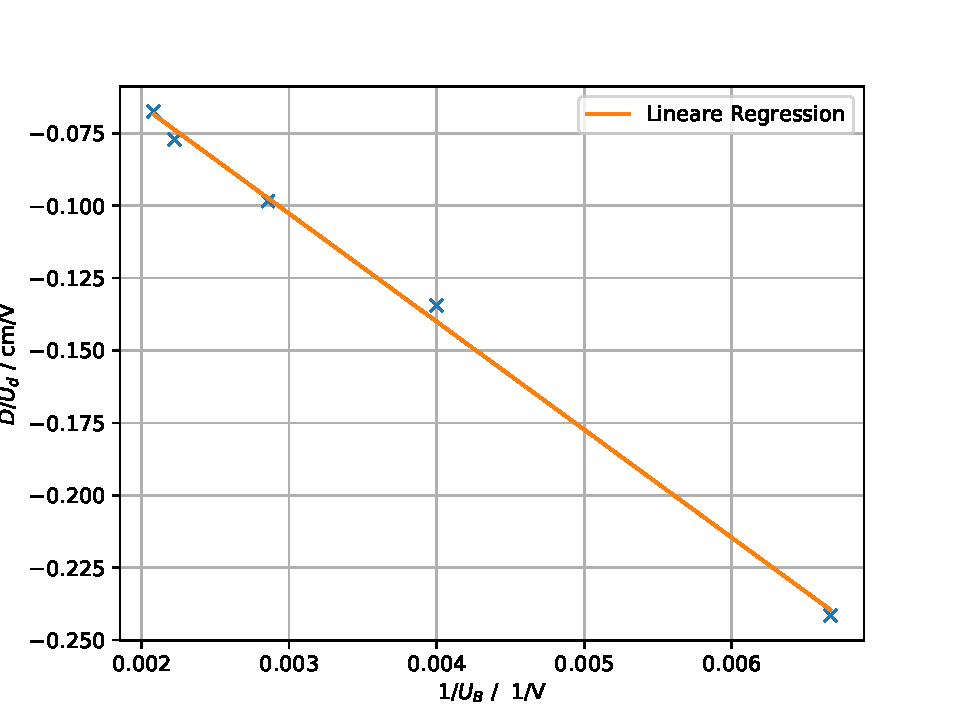
\includegraphics[width=0.8\textwidth]{Ergebniss.pdf}
  \caption{$D/U_{\text{d}}$ gegen $1/U_B$}
  \label{fig:Ergebniss}
\end{figure}
\\Die Steigung der Ausgleichsgraden beträgt:
\begin{equation*}
  a=\SI{0,3730 \pm 0,0115}{m}
\end{equation*}
\begin{align*}
  p=\SI{0,019}{m}\\
  d=\SI{0,0038}{m}\\
  L=\SI{0,1533}{m}\\
  \frac{pL}{2d}=\SI{0,38325}{m}
\end{align*}
\\Nun wird die Frequenz der Sinusspannung bestimmt. Als Beschleunigungsspannung wird $U_B=\SI{280}{V}$ verwendet.
Für bestimmte Frequenzen zeigt das Oszilloskop stehende Wellen an. Diese Frequenzen sind in der Tabelle \ref{tab:Frequenz} aufgeführt.
Der gemittelte Wert für $\nu_{\text{sin}}$ beträgt:
\begin{align*}
  \nu_{\text{sin}}=\SI{75,146}{Hz}.
\end{align*}
Die Amplitude der Sinusfrequenz beträgt ein Kästchen auf dem Gitternetz, das sind $D = \SI{0,635}{cm}$
Die Empfindlichkeit für $U_B=\SI{280}{V}$ wird über die Ausgleichsgrade in Abbildung \ref{fig:Ergebniss} ermittelt.
%\documentclass[captions=tableheading]{scrartcl}
%\usepackage{booktabs}
%\usepackage{pdflscape}


%\begin{document}
%\begin{landscape}




\begin{table}
  \centering
  \caption{Messdaten}
  \label{tab:Frequenz}
  \begin{tabular}{c c c}
    \toprule
    $n$ & $v/Hz$ & $v/Hz$\\

    \midrule
    3     &25     & 75\\
    1,5   &50,35  & 75\\
    1     &75,24  & 75\\
    0,75  &100,35 & 75\\
    0,6   &125,36 & 75\\
    0,5   &150,95 & 75\\
    0,4   &176,9  & 75\\
    \bottomrule
  \end{tabular}
\end{table}

%\end{landscape}
%\end{document}

\begin{align*}
  \frac{D_{\text{max}}}{U_{\text{sin}}}=\SI{0,1241}{\frac{cm}{V}}\\
  U_{\text{sin}} = \SI{5,1184}{V}
\end{align*}
\FloatBarrier
\subsection{Auswertung zu V502}
Das im Experiment verwendete Helmholtz-Spulenpaar hatte einen Radius von $R = \SI{0,282}{m}$ und $N=20$ Windungen.
In der Tabelle \ref{tab:V502} ist das aus der Stromstärke errechnete B-Feld für die gemessenen Spannungen und die Größe $\frac{D}{(D^2+L^2)}$ eingetragen. L ist dabei \SI{0,1533}{m}.
\documentclass[captions=tableheading]{scrartcl}
\usepackage{booktabs}
\usepackage{pdflscape}




\begin{document}
\begin{landscape}


\begin{table}
  \centering
  \caption{Messdaten}
  \label{tab:V502}
  \begin{tabular}{c c c c c c}
    \toprule
    $Höhe$ & $Strom_250$ & $Strom_300$ & $Strom_350$ & $Strom_400$ & $Strom_440$\\
    cm &   I &     I &    I &     I &    I   \\
    \midrule
      \documentclass[captions=tableheading]{scrartcl}
\usepackage{booktabs}
\usepackage{pdflscape}




\begin{document}
\begin{landscape}


\begin{table}
  \centering
  \caption{Messdaten}
  \label{tab:V502}
  \begin{tabular}{c c c c c c}
    \toprule
    $Höhe$ & $Strom_250$ & $Strom_300$ & $Strom_350$ & $Strom_400$ & $Strom_440$\\
    cm &   I &     I &    I &     I &    I   \\
    \midrule
      \documentclass[captions=tableheading]{scrartcl}
\usepackage{booktabs}
\usepackage{pdflscape}




\begin{document}
\begin{landscape}


\begin{table}
  \centering
  \caption{Messdaten}
  \label{tab:V502}
  \begin{tabular}{c c c c c c}
    \toprule
    $Höhe$ & $Strom_250$ & $Strom_300$ & $Strom_350$ & $Strom_400$ & $Strom_440$\\
    cm &   I &     I &    I &     I &    I   \\
    \midrule
      \input{V502.txt}
    \bottomrule
  \end{tabular}
\end{table}

\end{landscape}
\end{document}

    \bottomrule
  \end{tabular}
\end{table}

\end{landscape}
\end{document}

    \bottomrule
  \end{tabular}
\end{table}

\end{landscape}
\end{document}

Trägt man die Werte in Graphen ein und führt mit Python eine Ausgleichsrechnung durch, ergiben sich die Abbildungen  \ref{fig:1-250V}, \ref{fig:1-300V}, \ref{fig:1-350V}, \ref{fig:1-400V} und \ref{fig:1-450V}.
\begin{align*}
  m_{250V} =& \SI{11844,857\pm60,887}{\frac{1}{Tm}}\\
  Y_{250V} =& \SI{0,04214751\pm0,0005875}{m}\\
  m_{300V} =& \SI{10760,858\pm48,438}{\frac{1}{Tm}}\\
  Y_{300V} =& \SI{0,04691744\pm0,00056241}{m}\\
  m_{350V} =& \SI{10107,370\pm88,829}{\frac{1}{Tm}}\\
  Y_{350V} =& \SI{0,0615518\pm0,00114344}{m}\\
  m_{400V} =& \SI{ 9421,877\pm30,996}{\frac{1}{Tm}}\\
  Y_{400V} =& \SI{0,04504514\pm0,0004708}{m}\\
  m_{450V} =& \SI{ 8946,296\pm44,868}{\frac{1}{Tm}}\\
  Y_{450V} =& \SI{0,05506224\pm0,0005871}{m}
\end{align*}
\FloatBarrier
%\begin{figure}[h!]
%  \centering
%  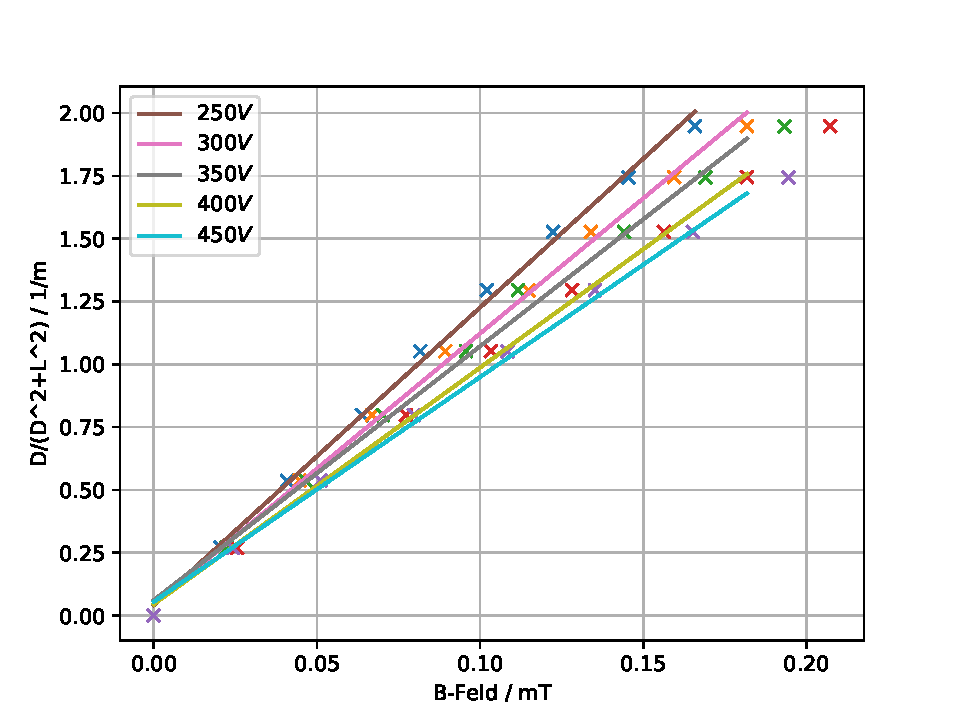
\includegraphics[width=0.8\textwidth]{V502.pdf}
%  \caption{$D/(D^2+L^2)$ gegen $B-Feld$}
%  \label{fig:V502}
%\end{figure}
\begin{figure}[h!]
 \centering
 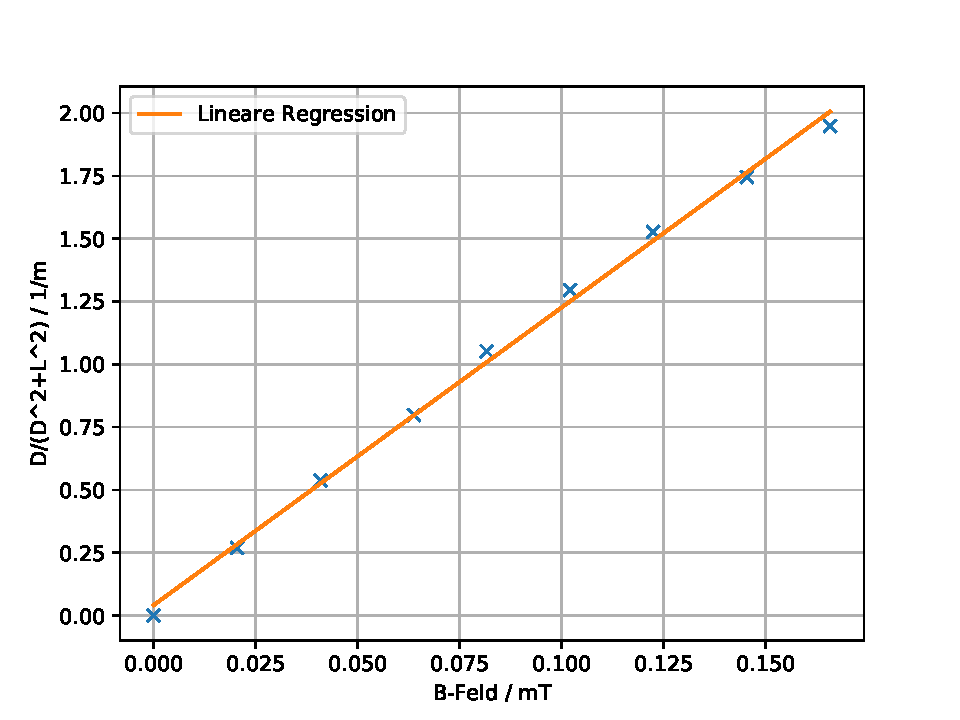
\includegraphics[width=0.8\textwidth]{1-250V.pdf}
 \caption{$D/(D^2+L^2)$ gegen $B-Feld f\ddot{u}r 250V$}
 \label{fig:1-250V}
\end{figure}
\begin{figure}[h!]
 \centering
 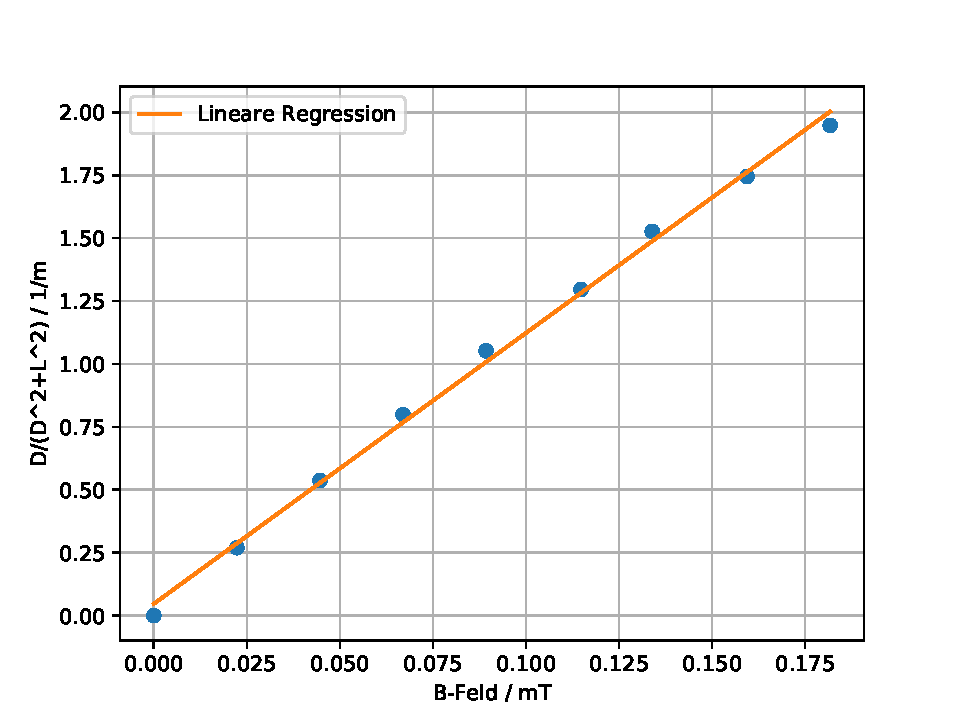
\includegraphics[width=0.8\textwidth]{1-300V.pdf}
 \caption{$D/(D^2+L^2)$ gegen $B-Feld f\ddot{u}r 300V$}
 \label{fig:1-300V}
\end{figure}
\begin{figure}[h!]
 \centering
 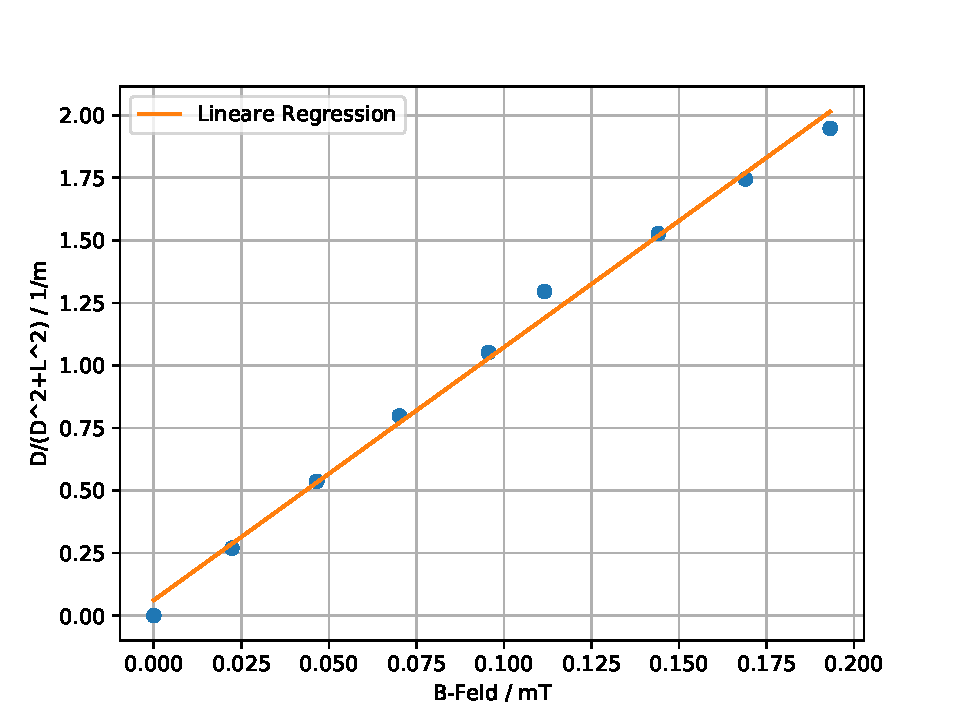
\includegraphics[width=0.8\textwidth]{1-350V.pdf}
 \caption{$D/(D^2+L^2)$ gegen $B-Feld f\ddot{u}r 350V$}
 \label{fig:1-350V}
\end{figure}
\begin{figure}[h!]
 \centering
 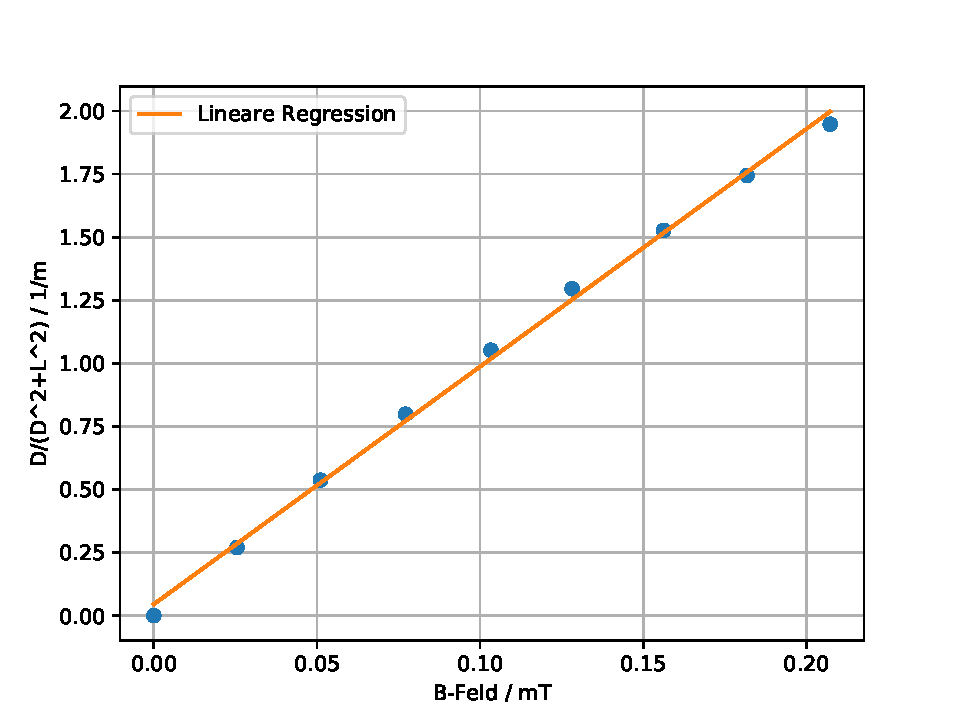
\includegraphics[width=0.8\textwidth]{1-400V.pdf}
 \caption{$D/(D^2+L^2)$ gegen $B-Feld f\ddot{u}r 400V$}
 \label{fig:1-400V}
\end{figure}
\begin{figure}[h!]
 \centering
 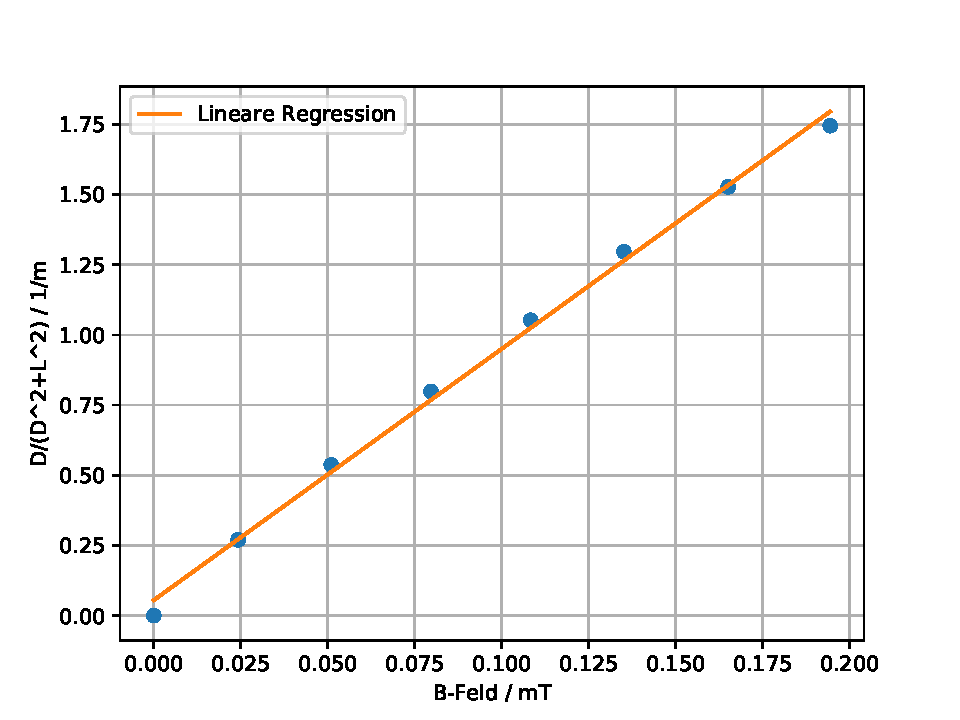
\includegraphics[width=0.8\textwidth]{1-450V.pdf}
 \caption{$D/(D^2+L^2)$ gegen $B-Feld f\ddot{u}r 450V$}
 \label{fig:1-450V}
\end{figure}
Aus den Graphiken werden folgende Steigungen und Y-Achsenabschnitte errechnet.
\\Mit den Steigungen lässt sich über die Gleichung \ref{eqn:e0m0} die Konstante $\frac{e_0}{m_0}$ bestimmen.
\FloatBarrier
Der Mittelwert liegt in etwa bei $\SI{2,82070789680e11}{\frac{C}{kg}}$
\begin{align*}
  U=&250V\\
  \frac{e_0}{m_0} =& \SI{2,806012747e11}{\frac{C}{kg}}\\
  U=&300V\\
  \frac{e_0}{m_0} =& \SI{2,779105558e11}{\frac{C}{kg}}\\
  U=&350V\\
  \frac{e_0}{m_0} =& \SI{2,860449993e11}{\frac{C}{kg}}\\
  U=&400V\\
  \frac{e_0}{m_0} =& \SI{2,840696519e11}{\frac{C}{kg}}\\
  U=&440V\\
  \frac{e_0}{m_0} =& \SI{2,817274667e11}{\frac{C}{kg}}\\
\end{align*}
Für die Berechnung des Erdmagnetfeldes werden die Werte
\begin{align*}
  I =\SI{ 0,26}{A}\\
  \varphi = \SI{72}{°}
\end{align*}
\\aufgenommen.
Mit den Formeln \ref{eqn:bhor} und \ref{eqn:btot} kann das totale Erdmagnetfeld berechnet werden:
\begin{equation*}
  B = \SI{0,053}{mT}.
\end{equation*}
\FloatBarrier
